As Artificial Intelligence (AI) is getting a greater impact in our everyday life, it is of utmost importance that it is safe for humans.  

One of the tools used in AI are deep neural networks (DNNs) and neural networks in general. Deep neural networks are powerful learning models that achieve excellent performance on visual recognition problems \cite{krizhevsky2012imagenet}. Those results imply that DNNs can be used in different industrial domains, e.g. traffic sign recognition, a domain in which DNNs even outperform humans \cite{outperformhumans}. 

Nevertheless, neural networks tend to have some peculiar properties as well. If only a few pixels in an image are changed, some neural networks produce incorrect results \cite{szegedy2013intriguing}. Such a behaviour is not desirable in safety-critical systems. For example, if an autonomous car recognizes a  \textit{STOP} sign as anything else but a \textit{STOP} sign, it can lead to deadly consequences. Therefore, it is important to verify the system. 

Three original and three adversarial samples that are crafted in one of the experiments this thesis is presented in Figure \ref{fig:motivational-samples}.

\begin{figure}

\begin{subfigure}{.5\textwidth}
  \centering
  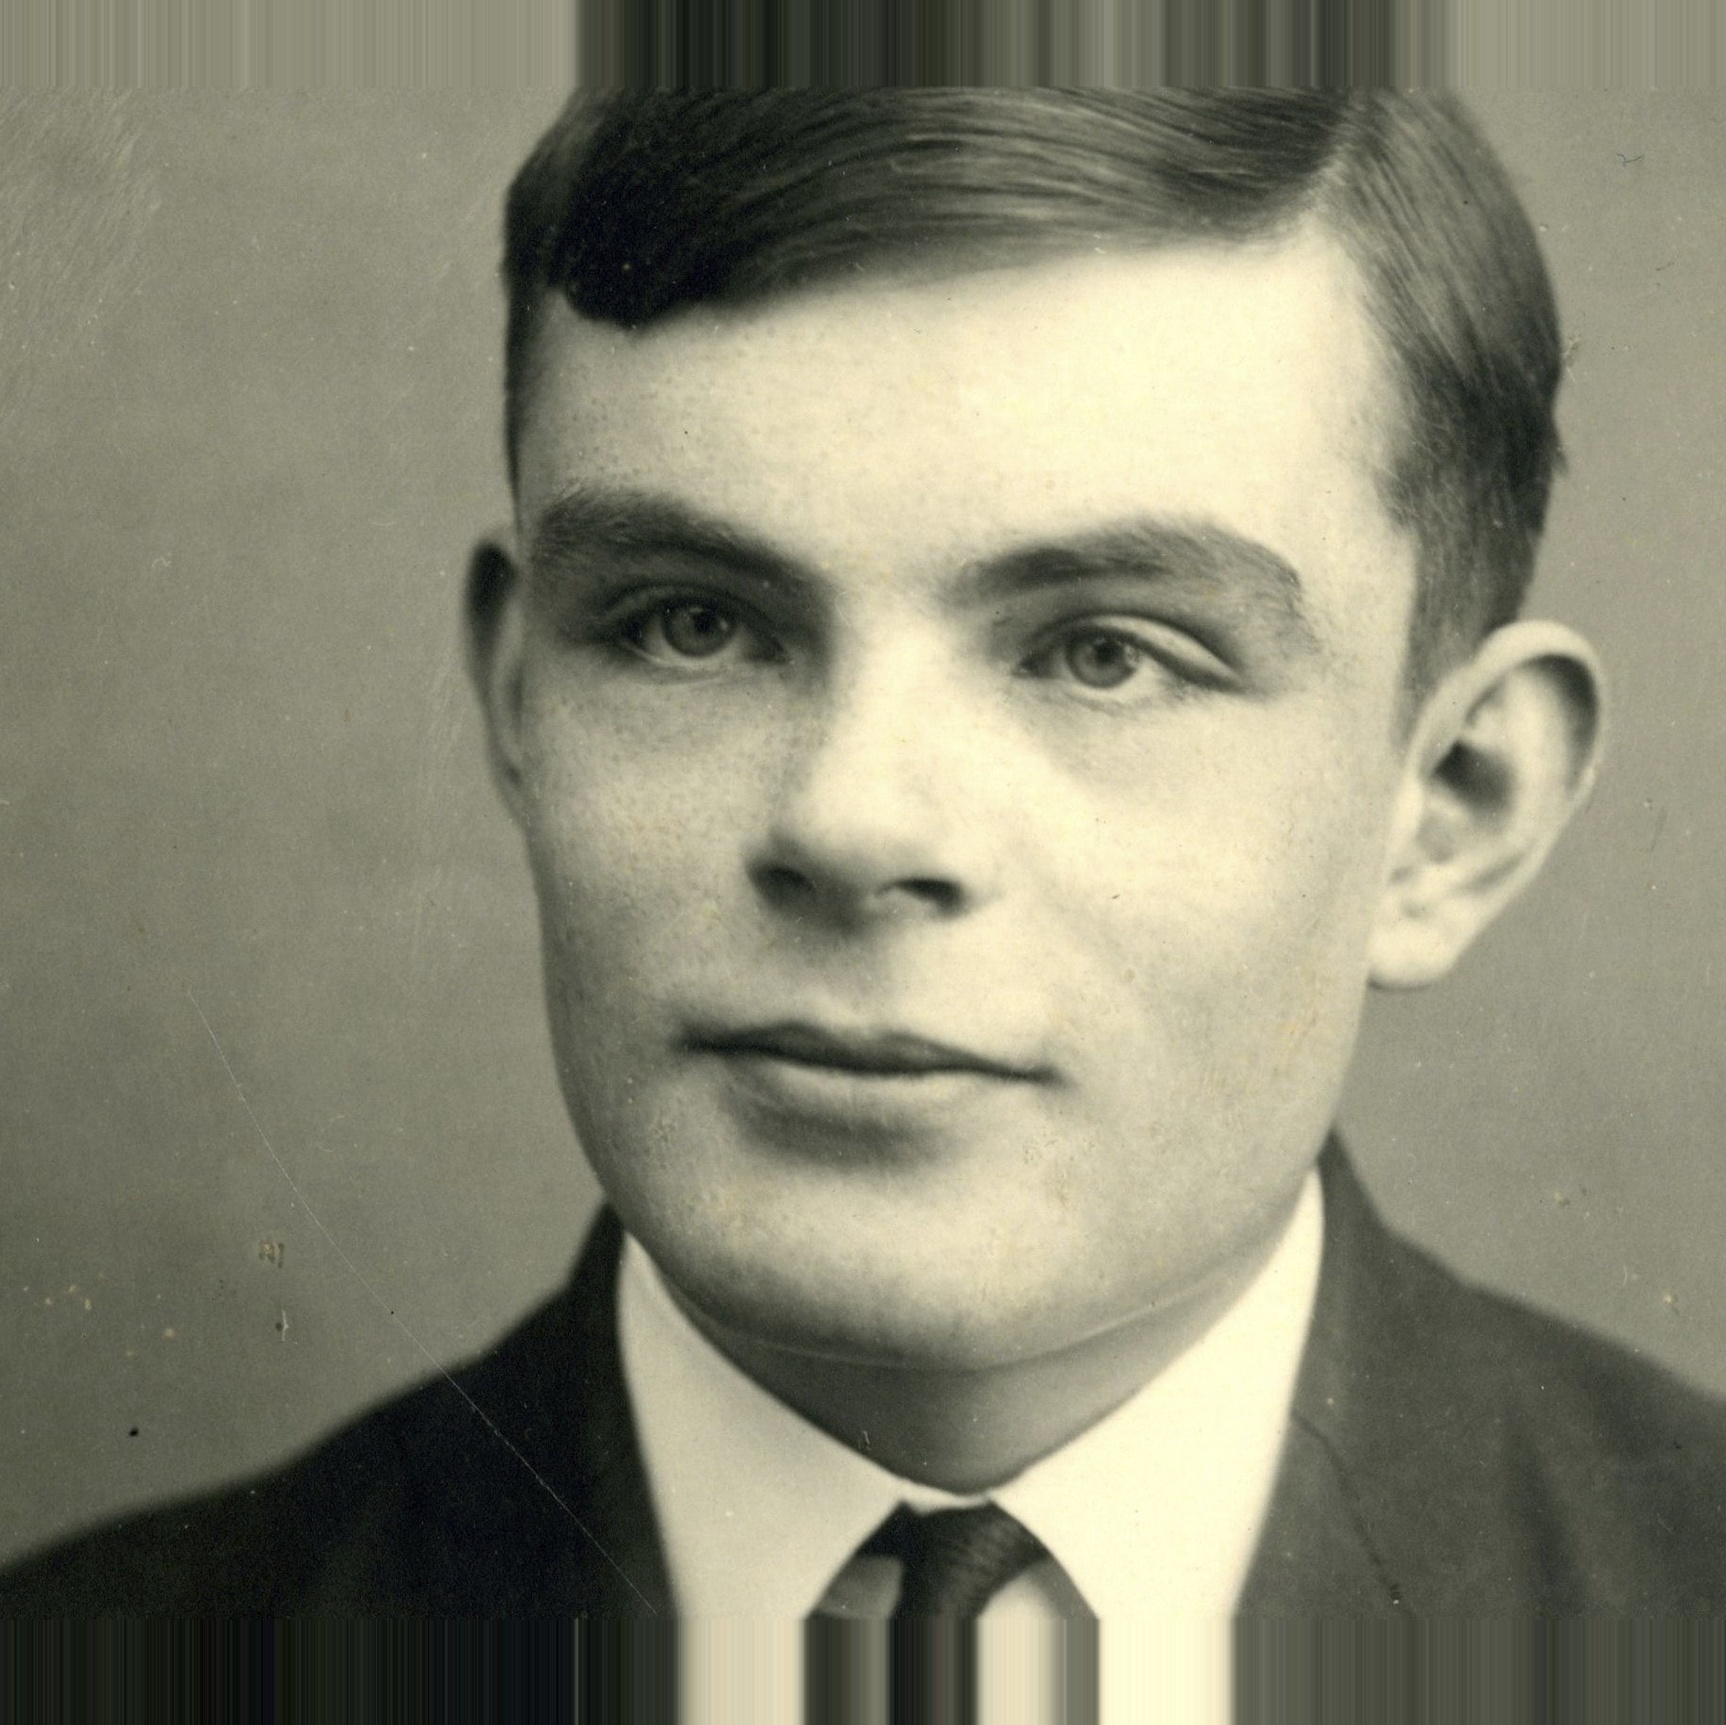
\includegraphics[height=5cm, width=\linewidth, keepaspectratio]{original_image_fgsm_1-eps1.jpg}
  \caption{Original sample classified as 28 years old}
\end{subfigure}
\begin{subfigure}{.5\textwidth}
  \centering
  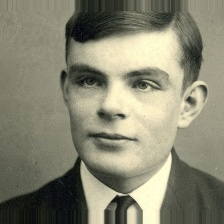
\includegraphics[height=5cm, width=\linewidth, keepaspectratio]{adversarial_image_fgsm_1-eps1.jpg}
  \caption{Adversarial sample classified as 59 years old}
\end{subfigure}

\begin{subfigure}{.5\textwidth}
  \centering
  
\includegraphics[height=5cm, width=\linewidth, keepaspectratio]{original_image_fgsm_2-eps1.jpg}
  \caption{Original sample classified as 59 years old}
\end{subfigure}
\begin{subfigure}{.5\textwidth}
  \centering
  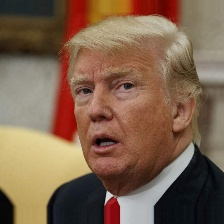
\includegraphics[height=5cm, width=\linewidth, keepaspectratio]{adversarial_image_fgsm_2-eps1.jpg}
  \caption{Adversarial sample classified as 28 years old}
\end{subfigure}

\begin{subfigure}{.5\textwidth}
  \centering
  
\includegraphics[height=5cm, width=\linewidth, keepaspectratio]{original_image_fgsm_3-eps1.jpg}
  \caption{Original sample classified as 28 years old}
\end{subfigure}
\begin{subfigure}{.5\textwidth}
  \centering
  
\includegraphics[height=5cm, width=\linewidth, keepaspectratio]{adversarial_image_fgsm_3-eps1.jpg}
  \caption{Adversarial sample classified as 64 years old}
\end{subfigure}

\caption{Original samples (left) and adversarial samples (right)}
\label{fig:motivational-samples}
\end{figure}

\section{Problem Definition} 
\label{motivation}
The assumption in the rest of this thesis is that the neural network is performing a \textit{classification task} - mapping an input (image) to a discrete output value (e.g. mapping an image of a traffic sign to the name of the traffic sign).  Output values are often called labels or categories. There is a finite number of possible labels.

To find errors in a system where a neural network is used, we need a framework which can trigger every possible output of the neural network.  We want to achieve that by using only one image as a starting point. 

Since for the same input we will always get the same output, modifications of that image are necessary. For each different desired output, a different modification of the image is performed.
Then we repeat that process by changing our desired output in every iteration and in that way, cover all possible outputs. The idea is that the modified image is as close as possible to the original one. For example, an image of a  \textit{STOP} sign can be modified as long as it still is an image of a  \textit{STOP} sign to a human observer. In that case, with the variations of the \textit{STOP} sign we cover all the possible outputs of the neural network - all other traffic signs. Using this technique, we can trigger errors in the system which can help us in the process of its verification. 

Modifying an input for a neural network with a goal of reaching an output that is different than the output of an unmodified input is an attack called \textit{misclassification}. If an output which an attacker wants to reach is one specific label, then a name of the attack is \textit{targeted misclassification}.

Creating a framework for targeted misclassification in the domain of age estimation as well as comparison and evaluation of existing approaches is the main focus of this thesis. In other words, the focus is on approaches how to trick a classifier to classify a person as older or younger than he or she actually is. 

\section{Aim of the Work}
To the best of my knowledge, nobody executed an attack against a DNN in the domain of age estimation yet. Hence, one of the first questions which this thesis aims to answer is the question whether already existing techniques can be used for attacks in this domain.

In order to further define aim of this work, an explanation of the major difference between two types of attacks against a neural network is necessary, namely the difference between \textit{white-box} attack and \textit{black-box} attack. 
In white-box attacks, an adversary has all the information about the DNN under attack. The internal structure of the neural network, all the implementation details and values of all the variables in any moment are known to the attacker. In other words, the attacker has access to the source code and nothing is hidden.
On the other hand, in black-box attacks an adversary doesn't have access to all the information. Depending on the precise definition of "black-box", more or less information is provided. In this thesis, the only capability of the black-box adversary is to observe the labels assigned by the DNN to chosen inputs.

A natural question is which algorithm is the best one for the white-box attack and which one for the black-box attack? Several algorithms are run in the different settings and results are compared. That provides an answer to the question which algorithm to use in which scenario.

Furthermore, in the domain of age estimation, it makes sense to be less strict about the targeted label. For instance, if an image of a minor is classified as an image of a person over a fifty years old, this could lead to the same consequences, no matter if it is classified as a 55 or 65 years old person. More precisely, if the goal is to hit any label from a specific group of labels, I define that attack as \textit{semi-targeted misclassification}. Of course, a group of labels must be smaller than a whole set of possible labels, otherwise the task is trivial. In general, this attack makes sense in any environment where labels can be clustered.

To this end, I adapted one already existing black-box approach is adapted to this more relaxed setting. Such a relaxation is not yet introduced in the literature since it is very domain specific. Consequently, the results can't be compared against previous work of that kind, but results are compared with targeted black-box misclassification attacks. This comparison is explained in more details in Section \ref{approach}. 

In terms of development, a DNN is implemented which receives an image as an input and outputs how old the person in the image is. In other words, a DNN for age estimation is trained. All the attacks are executed against this DNN. 

Next, the framework is constructed for a white-box and a black-box targeted misclassification attack. In other words, while treating the DNN as a white-box or a black-box, images  are constructed in a way that the targeted DNN outputs a specific year. Finally, the framework is extended with capability to craft semi-targeted black-box misclassification attacks.

\section{Methodological Approach} \label{approach}
The methodological approach consists of the following steps:
\begin{enumerate}
    \item I write about the background knowledge needed for training a neural network. The goal is to give a brief introduction to this area so that a non-expert reader can follow the rest of the thesis. Using that knowledge, I trained a deep neural network for age estimation of a person in the image.
    
    \item I conducted a research about different state of the art methods for generating \textit{adversarial examples}, i.e. images which are not correctly classified by DNN. The focus here is on the approaches that address targeted misclassification. While treating a DNN from the first step as a white-box, I use those methods to construct adversarial examples. Afterwards, I present and analyze the results of the attacks.
    
    \item I did a literature survey on the targeted black-box attack methods, explain those methods and use them to generate adversarial inputs for a DNN  from the first step, but this time while treating it as a black box. I compare the results of different algorithms.
    
    \item As the last step, combining the domain knowledge and an existing attack method, I implemented a new adversarial algorithm and using that algorithm, I construct images for semi-targeted misclassification. I compare results against targeted black-box approaches. The way I is compared them is the following: a target label for a targeted version of the attack is the median value of the set of labels in a semi-targeted version of the attack. If a DNN outputs any label outside the set of the labels, an attack is  considered as a successful no matter if it is a targeted or a semi-targeted misclassification attack.
\end{enumerate}


\section{Outline} 
In this chapter an introduction to the problem is provided. In the next chapter background knowledge is presented that is needed to follow the rest of the thesis. In Chapter \ref{chap:attacks} state-of-the-art attacks are presented and explained. In Chapter \ref{chap:experiments} results of the experiments are presented. The Semi-Targeted Approach is discussed in Chapter \ref{chap:semi-targeted}. Threats to validity and ideas for future work are presented in Chapter \ref{chap:threats}. Finally, summary of this thesis is presented in Chapter \ref{chap:summary}.

